\documentclass{article}[a4paper]
\usepackage[a4paper, total={6.5in, 9.5in}]{geometry}
\usepackage{charter}
\usepackage{xcolor}
\usepackage{graphicx}
\usepackage{float}
\usepackage{listings}
\usepackage{tabularray}
\usepackage{amsmath}
\usepackage{amssymb}
\usepackage[hidelinks]{hyperref}

\lstset{
  language=Python,
  basicstyle=\ttfamily,
  keywordstyle=\color{blue},
  commentstyle=\color{gray},
  stringstyle=\color{red},
  showstringspaces=false,
  columns=fullflexible,
  breaklines=true
}

\title{
	\huge{\textbf{
		Assignment 01
	}}\\
	\Large{
		Learning from Data, Related Challenges, Linear Models for Regression
	}\\
	\large{\phantom{}}\\
	\large{
		submitted for
	}\\
	\LARGE{
		\textbf{EN3150 - Pattern Recognition}
	}\\
	\large{
		Department of Electronic and Telecommunication Engineering
	}
	\\
	\large{University of Moratuwa}
}

\author{
	\textbf{Udugamasooriya P. H. J.}\\
	220658U % \quad - \quad \href{https://github.com/pulasthi-u/en3160-assignment01}{GitHub}\\
}

\date{12 August 2025}

\allowdisplaybreaks

\begin{document}

	\maketitle

	\section{Impact of Outliers on Linear Regression}

	\textbf{Question 02}
	We start by representing the independent in a matrix \[
		\mathbf{X} = \begin{pmatrix}
			1		& x_1		\\
			\vdots	& \vdots	\\
			1		& x_n
		\end{pmatrix},
	\] and the dependent variables in a vector \[
		\mathbf{y} = \begin{pmatrix}
			y_1 & \cdots & y_n
		\end{pmatrix} ^ \top,
	\] and look for a vector of weights $\mathbf{w}_\text{OLS} = \begin{pmatrix} w_0 & w_1 \end{pmatrix} ^ \top$ such that \[
		\mathbf{w}_\text{OLS}
		=
		\underset{\mathbf{w}}{\arg\min}
		\left( \mathbf{y} - \mathbf{X} \mathbf{w} \right)^2.
	\] We directly use the result that \[
		\mathbf{w}_\text{OLS}
		=
		\left( \mathbf{X}^\top \mathbf{X} \right)^{-1} \mathbf{X}^\top \mathbf{y}.
	\] We implement exactly what is described above in code, and obtain the following result:
	\begin{lstlisting}
Ordinary Least Squares Weights (w): [ 3.91672727 -3.55727273]
	\end{lstlisting}
	Hence \[
		\mathbf{w}_\text{OLS} = \begin{pmatrix} 3.91672727 \\ -3.55727273 \end{pmatrix},
	\] and the predicted linear model is \[
		y = 3.91672727 - 3.55727273 x.
	\]
	A plot of the given data points against the predicted values is shown in Figure \ref{q1}.

	\begin{figure}[H]
		\centering
		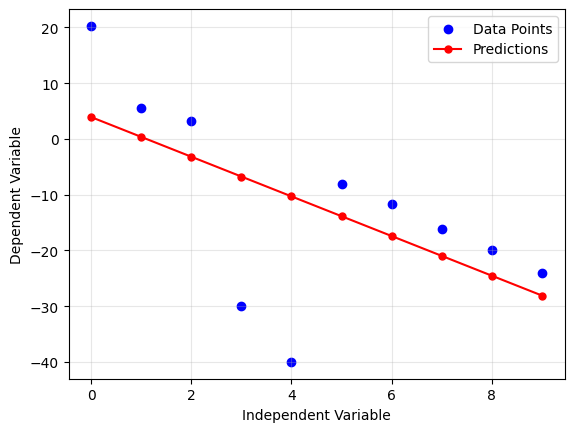
\includegraphics[width=0.7\linewidth]{images/q1.png}
		\caption{abc}
		\label{q1}
	\end{figure}

	\textbf{Question 04} abc
	
	\textbf{Question 05} pqr

	\textbf{Question 06} xyz

	\textbf{Question 07} def

	\textbf{Question 08} ghi

	\section{Loss Functions}

	\textbf{Question 01} We calculate the squared error \[
		\text{SE}(\hat{y}_i, y_i) = (\hat{y}_i - y_i)^2
	\] and binary cross entropy \[
		\text{BCE}(\hat{y}_i, y_i) = -y_i \log(\hat{y}_i) - (1 - y_i) \log(1 - \hat{y}_i)
	\] of each predicted value $\hat{y}_i$ against the given corresponding target value $y_i$.
	\newline

	\begin{tblr}{
		colspec={X[1, c] X[1, c] X[1, c] X[1, c]},
		vlines, hlines
	}
		True Value ($y_i$)	& Predicted Value ($\hat{y}_i$)	& $\text{SE}(\hat{y}_i, y_i)$	& $\text{BCE}(\hat{y}_i, y_i)$ \\
		1 					& 0.005 						& 0.9900 						& 5.2983 \\
		1 					& 0.010 						& 0.9801 						& 4.6052 \\
		1 					& 0.050 						& 0.9025 						& 2.9957 \\
		1 					& 0.100 						& 0.8100 						& 2.3026 \\
		1 					& 0.200 						& 0.6400 						& 1.6094 \\
		1 					& 0.300 						& 0.4900 						& 1.2040 \\
		1 					& 0.400 						& 0.3600 						& 0.9163 \\
		1 					& 0.500 						& 0.2500 						& 0.6931 \\
		1 					& 0.600 						& 0.1600 						& 0.5108 \\
		1 					& 0.700 						& 0.0900 						& 0.3567 \\
		1 					& 0.800 						& 0.0400 						& 0.2231 \\
		1 					& 0.900 						& 0.0100 						& 0.1054 \\
		1 					& 1.000 						& 0.0000 						& 0.0000 \\
							& Mean							& 0.4402		 				& 1.4407
	\end{tblr}
	\newline
	
	A plot of the different losses against the predicted values is shown in Figure \ref{q2}.

	\begin{figure}[H]
		\centering
		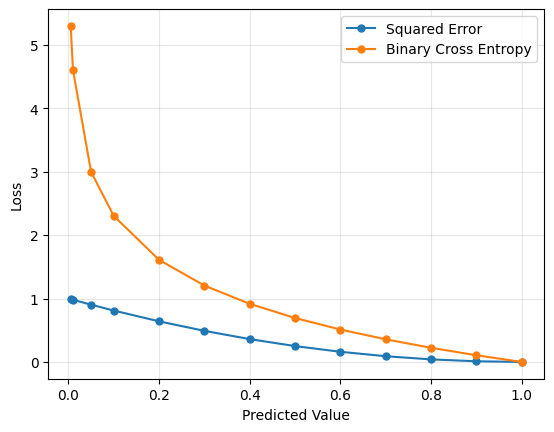
\includegraphics[width=0.7\linewidth]{images/q2.png}
		\caption{abc}
		\label{q2}
	\end{figure}

	\textbf{Question 02}

	\section{Data Pre-Processing}

	\textbf{Question 01}

\end{document}